\documentclass[11pt]{article}

\usepackage[T1]{fontenc}
\usepackage{geometry}
\usepackage{amsmath, amssymb, amsthm}
\usepackage[scr]{rsfso}
\usepackage[%
    hidealllines=true,%
    innerbottommargin=15,%
    nobreak=true,%
]{mdframed}
\usepackage{bm}
\usepackage{xcolor}
\usepackage{graphicx}
\usepackage{fancyhdr}
\usepackage{hyperref}

\geometry{a4paper, margin=1in, headheight=14pt}

\pagestyle{fancy}
\fancyhf{}
\renewcommand\headrulewidth{0.4pt}
\fancyhead[L]{\scshape MA3102: Algebra I}
\fancyhead[R]{\scshape \leftmark}
\rfoot{\footnotesize\it Updated on \today}
\cfoot{\thepage}

\newcommand{\C}{\mathbb{C}}
\newcommand{\R}{\mathbb{R}}
\newcommand{\Q}{\mathbb{Q}}
\newcommand{\Z}{\mathbb{Z}}
\newcommand{\N}{\mathbb{N}}

\renewcommand{\vec}[1]{\boldsymbol{#1}}
\newcommand{\vv}{\vec{v}}
\newcommand{\vw}{\vec{w}}
\newcommand{\vx}{\vec{x}}
\newcommand{\vy}{\vec{y}}
\newcommand{\ve}{\vec{e}}
\newcommand{\va}{\vec{a}}
\newcommand{\vb}{\vec{b}}

\newcommand{\norm}[1]{\Vert #1 \Vert}
\newcommand{\ip}[2]{\langle #1, #2 \rangle}

\newcommand{\im}{\operatorname{im}}
\newcommand{\sign}{\operatorname{sgn}}
\newcommand{\aut}{\operatorname{Aut}}

\newmdtheoremenv[%
    backgroundcolor=blue!10!white,%
]{theorem}{Theorem}[section]
\newmdtheoremenv[%
    backgroundcolor=violet!10!white,%
]{corollary}{Corollary}[theorem]
\newmdtheoremenv[%
    backgroundcolor=teal!10!white,%
]{lemma}[theorem]{Lemma}

\theoremstyle{definition}
\newmdtheoremenv[%
    backgroundcolor=green!10!white,%
]{definition}{Definition}[section]
\newmdtheoremenv[%
    backgroundcolor=red!10!white,%
]{exercise}{Exercise}[section]

\theoremstyle{remark}
\newtheorem*{remark}{Remark}
\newtheorem*{example}{Example}
\newtheorem*{solution}{Solution}

\surroundwithmdframed[%
    linecolor=black!20!white,%
    hidealllines=false,%
    innertopmargin=5,%
    innerbottommargin=10,%
    skipabove=0,%
    skipbelow=0,%
]{example}

\numberwithin{equation}{section}

\title{
    \Large\textsc{MA3102} \\
    \Huge \textbf{Algebra I} \\
    \vspace{5pt}
    \Large{Autumn 2021}
}
\author{
    \large Satvik Saha
    \\\textsc{\small 19MS154}
}
\date{\normalsize
    \textit{Indian Institute of Science Education and Research, Kolkata, \\
    Mohanpur, West Bengal, 741246, India.} \\
}

\begin{document}
    \maketitle

    \tableofcontents

    \section{Symmetries}
    \subsection{Symmetries of plane figures}
    A symmetry of a plane figure can be thought of as a rigid motion which
    \emph{preserves its structure}, i.e.\ sends it to itself.

    For example, consider an equilateral triangle; there is the identity symmetry
    (which does nothing), two rotations by $2\pi / 3$ and $2\pi / 3$, and three
    reflections. This gives us a total of $6$ symmetries. Coincidentally, the plane
    symmetries of an equilateral triangle are precisely the set of $3! = 6$
    permutations of its vertices.

    \begin{center}
        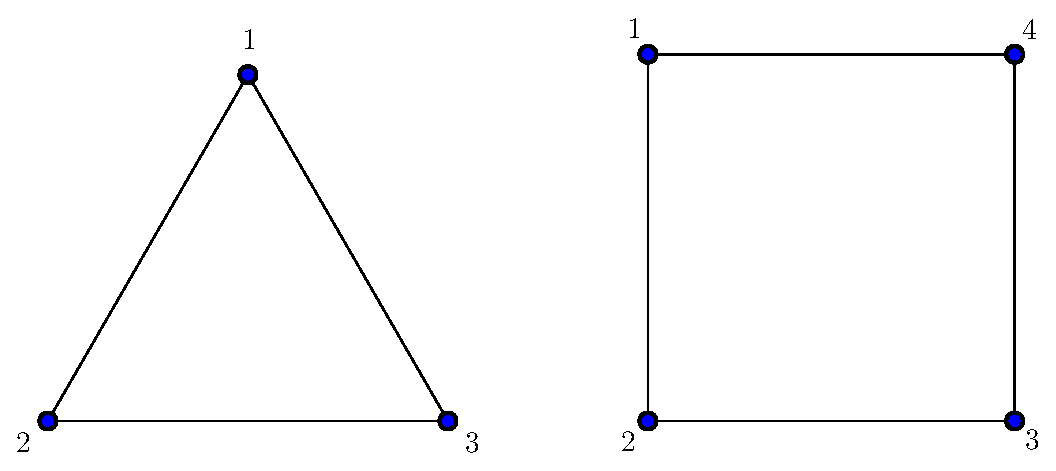
\includegraphics[width=0.6\textwidth]{./triangle_square.eps}
    \end{center}

    The same cannot be said of a square; there are $4! = 24$ of its vertices, but
    only $8$ of them are rigid motions. Here, we see $4$ rotations and $4$
    reflections.

    In general, a regular $n$-gon has $2n$ plane symmetries, of which $n$ are
    rotations and $n$ are reflections. This can be seen by noting that a symmetry of
    an $n$-gon is completely determined by its action on an edge; once the final
    positions of the first two vertices is determined, the rest are forced. There are
    $n$ positions for the first vertex, which leaves only $2$ positions for the
    second vertex. One of these choices results in a rotation (since it preserves the
    cyclicity of the vertices) and the other a reflection (since it reverses the
    cyclicity of the vertices).

    Note that these symmetries can be \emph{composed}, i.e.\ applied in succession.
    For example, a rotation by $2\pi / n$ can be applied repeatedly to obtain every
    possible rotational symmetry. Similarly, we can perform rotations and reflections
    in succession, and we always end up with another symmetry. This composition is
    associative, there is an identity symmetry, and each symmetry has an inverse.
    The collection of such symmetries forms a \emph{group}.

    The group of plane symmetries of a regular $n$-gon is called the \emph{dihedral
    group}, denoted as $D_{2n}$.

    \subsection{Symmetries of the Euclidean plane}
    Consider the class of isometries of the plane, i.e.\ all bijections $f\colon \R^2
    \to \R^2$ such that $\norm{f(\vv) - f(\vw)} = \norm{\vv - \vw}$. These constitute
    symmetries of the Euclidean plane $\R^2$. The three basic forms of such
    symmetries are rotations, reflections, and translations; it can be shown that
    every symmetry of $\R^2$ is a combination of at most three reflections.  Another
    representation for each symmetry is \[
        f(\vv) = A\vv + \vv_0,
    \] where $A \in O_2(\R)$ is an orthogonal matrix, accounting for the rotational
    and reflectional part of the transformation.

    To show this, set $\vv_0 = f(\vec{0})$ and define $g = f - \vv_0$. Thus,
    $g(\vec{0}) = \vec{0}$, and $g$ is also an isometry.
    
    Not that for all $\vv, \vw \in \R^2$, we can write
    \begin{align*}
        \norm{g(\vv) - g(\vw)}^2 &= \norm{g(\vv)}^2 + \norm{g(\vw)}^2 -
        2\ip{g(\vv)}{g(\vw)}, \\
        \norm{\vv - \vw}^2 &= \norm{\vv}^2 + \norm{\vw}^2 -
        2\ip{\vv}{\vw}.
    \end{align*}
    On the other hand, $\norm{g(\vv) - g(\vw)}^2 = \norm{\vv - \vw}^2$, and
    $\norm{g(\vv)}^2 = \norm{\vv}^2$, $\norm{g(\vw)}^2 = \norm{\vw}^2$. This gives
    $\ip{g(\vv)}{g(\vw)} = \ip{\vv}{\vw}$, i.e.\ $g$ preserves the inner product.

    We claim that $g(\alpha\vv) = \alpha g(\vv)$ for all $\alpha \in \R$, $\vv
    \in \R^2$. Note that $\norm{g(\alpha\vv)} = \norm{\alpha\vv} = \norm{\alpha g(\vv)}$.
    Now,
    \begin{align*}
        \norm{g(\alpha\vv) - \alpha g(\vv)}^2 &= \norm{g(\alpha\vv)}^2 + \norm{\alpha
        g(\vv)}^2 - 2\ip{g(\alpha\vv)}{\alpha g(\vv)} \\
        &= \alpha^2v^2 + \alpha^2v^2 - 2\alpha\ip{\alpha\vv}{\vv} \\
        &= 2\alpha^2v^2 - 2\alpha^2v^2 \\
        &= 0.
    \end{align*}    
    This proves that $g(\alpha\vv) = \alpha g(\vv)$.

    Next, we claim that $g(\vv + \vw) = g(\vv) + g(\vw)$ for all $\vv, \vw \in
    \R^2$. Write
    \begin{align*}
        \norm{g(\vv + \vw) - g(\vv) - g(\vw)}^2 &= \norm{g(\vv + \vw) - g(\vv)}^2 +
        \norm{g(\vw)}^2 - 2\ip{g(\vv + \vw) - g(\vv)}{g(\vw)} \\
        &= \norm{\vv + \vw - \vv}^2 + \norm{\vw}^2 - 2\ip{\vv + \vw}{\vw} +
        2\ip{\vv}{\vw} \\
        &= w^2 + w^2 - 2\ip{\vv}{\vw} - 2w^2 + 2\ip{\vv}{\vw} \\
        &= 0.
    \end{align*}
    This proves that $g(\vv + \vw) = g(\vv) + g(\vw)$. Thus, $g$ is a linear map.

    Now let $g(\ve_1) = \va$ and $g(\ve_2) = \vb$. Clearly, $\norm{\va} = \norm{\vb}
    = 1$. For arbitrary $\vv\in \R^2$, we immediately get $g(\vv) = v_x\va + v_y\vb$,
    so by arranging $\va$ and $\vb$ as the columns of a $2\times 2$ matrix $A$, we
    have $g(\vv) = A\vv$. We clearly have $A^\top A = \mathbb{I}_2$ from $\va^\top\va
    = \vb^\top\vb = 1$, and $\ip{\va}{\vb} = \ip{\ve_1}{\ve_2} = 0$. Thus, $A \in
    O_2(\R)$. Substituting this back into $f$, we have \[
        f(\vv) = A\vv + \vv_0
    \] as desired.

    It can be further shown (algebraically) that every member of $O_2(\R)$ is of the
    form \[
        \begin{bmatrix}
            \cos\theta & \mp\sin\theta \\ \sin\theta & \pm \cos\theta
        \end{bmatrix}.
    \] 


    \subsection{Symmetries of the Petersen graph}
    Consider a graph $G(V, E)$. A symmetry of $G$ is a bijection $f\colon V \to V$
    on the set of vertices, which preserves the edges. In other words, it preserves
    the adjacency function. Thus, it can be shown that the degree of each vertex will
    be preserved by a symmetry.

    The following graph is called the Petersen graph, with 10 vertices and 15 edges.

    \begin{center}
        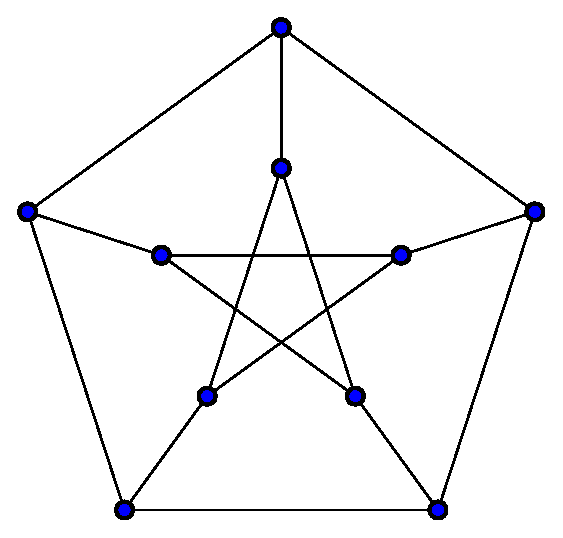
\includegraphics[width=0.5\textwidth]{./petersen.eps}
    \end{center}

    We can show that this graph has $120$ symmetries. This can be done by looking at
    all $2$ element subsets of $\{1, 2, 3, 4, 5\}$, of which there are $10$. Place
    these subsets as the vertices of a new graph, and connect two such sets with an
    edge if they \emph{are disjoint}. The resulting graph can be shown to be
    identical to the Petersen graph. It is immediately clear that any permutation of
    the set $\{1, 2, 3, 4, 5\}$ produces a relabelling of the vertices, which
    nevertheless preserves the Petersen graph. This gives us at least $5! = 120$
    symmetries.

    To show that there are at most $120$ symmetries, note that every vertex has
    exactly 3 neighbours. Thus, when sending a vertex $V$ to its image, we have $10$
    choices, but we have $3$ choices for the first neighbour $V_1$, $2$ for the
    second neighbour $V_2$. and $1$ for the third neighbour $V_3$. Finally, choose a
    neighbour of $V_3$, say $V_4$ and place it in on of the $2$ remaining positions.
    It can be shown that this completely determines the symmetry; each remaining
    vertex has a complete characterization in terms of the ones already fixed. Thus,
    we have an upper bound of $10 \times 3 \times 2 \times 1 \times 2 = 120$
    symmetries.
    

    \section{Groups}
    \subsection{Basic definitions}

    \begin{definition}
        A group is a set $G$ equipped with a binary operation, satisfying the
        following properties.
        \begin{enumerate}
        \itemsep0em
            \item \emph{Associativity}: For all $x, y, z \in G$, $x(yz) = (xy)z$.
            \item \emph{Existence of an identity element}: There exists $e \in G$
            such that for all $x \in G$, $ex = e = xe$.
            \item \emph{Existence of inverse elements}: For every $x \in G$, there
            exists some $y \in G$ such that $xy = e = yx$. We denote $y = x^{-1}$.
        \end{enumerate}
    \end{definition}
    \begin{example}
        The integers $\Z$ form a group under addition.
    \end{example}
    \begin{example}
        The set $\{-1, +1\}$ forms a group under multiplication.
    \end{example}
    \begin{example}
        The symmetries of a tetrahedron form a group under composition of symmetries.
    \end{example}

    \begin{lemma}
        The identity element in a group is unique.
    \end{lemma}
    \begin{proof}
        Let $G$ be a group, and suppose that $e, e' \in G$ satisfy \[
            ex = x = xe, \qquad e'x = x = xe'
        \] for all $x \in G$. Thus, we specifically have \[
            ee' = e' = e'e, \qquad e'e = e = ee',
        \] hence $e = e'$.
    \end{proof}

    \begin{lemma}
        The inverse of an element in a group is unique.
    \end{lemma}
    \begin{proof}
        Let $G$ be a group, and let $x \in G$. Suppose that $y, y' \in G$ satisfy \[
            xy = e = yx, \qquad xy' = e = y'x.
        \] Thus \[
            y = ye = y(xy') = (yx)y' = ey' = y'. \qedhere
        \] 
    \end{proof}

    \begin{lemma}
        The inverse of the inverse of an element in a group is the element itself.
    \end{lemma}
    \begin{proof}
        Let $G$ be a group, and let $x \in G$. Set $w = (x^{-1})^{-1}$. We have \[
            x^{-1}x = e = x x^{-1}, \qquad wx^{-1} = e = x^{-1}w.
        \] Thus, \[
            w = we = w(x^{-1}x) = (wx^{-1})x = ex = x. \qedhere
        \] 
    \end{proof}

    \begin{lemma}[Cancellation Law]
        Let $G$ be a group, and let $x, a, b \in G$ such that $xa = xb$. Then, $a =
        b$. Analogously, if $ax = bx$, then $a = b$.
    \end{lemma}
    \begin{proof}
        Simply multiply by $x^{-1}$ as appropriate.
    \end{proof}

    \begin{definition}
        The order of a group $G$ is the number of elements it contains, i.e.\ $|G|$.
        The order of an element $g \in G$ is the smallest possible natural number $n$
        such that $g^n = e$.
    \end{definition}

    \subsection{Subgroups}

    \begin{definition}
        Let $G$ be a group, and let $H \subseteq G$. We call $H$ a subgroup of $G$ if
        \begin{enumerate}
        \itemsep0em
            \item $e \in H$.
            \item For all $x, y \in H$, $xy \in H$.
            \item For all $x \in H$, $x^{-1} \in H$.
        \end{enumerate}
        Note that this is enough to guarantee that $H$ is a group under the same
        group operation as $G$.
    \end{definition}
    \begin{example}
        Consider the group $\C\setminus\{0\}$ of non-zero complex numbers under
        multiplication. The non-zero reals $\R\setminus\{0\}$ form a subgroup of this
        group.
    \end{example}

    \begin{theorem}
        Let $\Z$ be the group of integers under addition. Then, every subgroup of
        $\Z$ is of the form $\{0\}$ or $n\Z = \{nk: k \in \Z\}$.
        \begin{remark}
            The same argument shows that every subgroup of a cyclic group is cyclic.
        \end{remark}
    \end{theorem}
    \begin{proof}
        Let $H \subseteq \Z$ be a subgroup. If $H = \{0\}$, we are done. Otherwise,
        $H$ contains some positive integers; this is clear since $H$ must contain
        some non-zero integers, whose inverses have the opposite sign. Let $n \in H$
        be the smallest positive integer; we immediately have $n\Z \subseteq H$. Now
        let $m \in H$ be any other element.  Now, use Euclid's Division Lemma to
        write $m = nq + r$, where $0 \leq r < n$.  Now, note that $n \in H$ implies
        that $nq \in H$, hence the quantity $r = m - nq \in H$. The minimality of $n$
        forces $r = 0$, hence $m = nq$. This gives $H \subseteq n\Z$.
    \end{proof}
    \begin{corollary}
        If $a$ and $b$ are coprime integers, there exist integers $m$ and $n$ such
        that $am + bn = 1$.
    \end{corollary}
    \begin{proof}
        If $a$ and $b$ are coprime, they share no common factors greater than $1$.
        Note that $a\Z + b\Z$ is a subgroup of the integers, and hence there is
        exists a unique positive integer $d$ such that $a\Z + b\Z = d\Z$. Since $a, b
        \in a\Z + b\Z$, we have $a, b \in d\Z$ so there exist $r_1$, $r_2$ such that
        $a = dr_1$, $b = dr_2$. This means that $d$ is a common factor of $a$ and
        $b$, forcing $d = 1$, i.e.\ $a\Z + b\Z = \Z$. Since $1 \in \Z$, $1 \in
        a\Z + b\Z$, hence there exists a combination $am + bn = 1$.
    \end{proof}
    \begin{corollary}
        The unique positive integer $d$ such that $a\Z + b\Z = d\Z$ is the greatest
        common divisor of $a$ and $b$.
    \end{corollary}
    \begin{proof}
        Let $d$ be the greatest common divisor of $a$ and $b$. Write $a = a'd$, $b =
        b'd$, and note that $a'$ and $b'$ are coprime. Thus, pick $m$ and $n$ such
        that $a'm + b'n = 1$. This gives $d = am + bn$, so $d\Z \subseteq a\Z + b\Z$.
        Now, consider an arbitrary combination $ap + bq \in a\Z + b\Z$; simply write
        $ap + bq = (a'p + b'q)d \in d\Z$, hence $a\Z + b\Z \subseteq d\Z$.
    \end{proof}

    \begin{theorem}
        Let $\C^\times$ be the group of non-zero complex numbers under
        multiplication. Then, every finite subgroup of $\C^\times$ is of the form
        $H_n = \{z^k : k \in \N\}$ for some $n$\textsuperscript{th} root of unity
        $z$.
    \end{theorem}
    \begin{proof}
        Let $H \subset \C^\times$ be a finite subgroup. Note that we demand $1 \in
        H$. If this is the only element of $H$, we are done, otherwise choose a
        different $z \in H$. Now, if $|z| \neq 1$, note that there are infinitely
        many elements $z, z^2, z^3, \dots$ which must belong to $H$, which is a
        contradiction; note that these generated elements are distinct as they have
        different magnitudes. Thus we demand $|z| = 1$, so write $e^{2\pi ix}$.

        Examine the elements $1, z, z^2, \dots, z^n, \dots \in H$ for all $n \in \N$.
        Since $H$ is finite, some pair of these must be equal. This means that $z^a =
        z^b$ for some $a < b$, so cancellation gives $z^{b - a} = 1$. Thus, $z$ is a
        root of unity, which means that $z = e^{2\pi i k / n}$ for some $n
        \in \N$, $0 < k < n$.

        We have shown that every non-identity element in $H$ is a root of unity.
        Thus, pick $w = e^{2\pi ix} \in H$ such that $0 < x < 1$ and $x$ is minimal.
        Furthermore, set $x = k / n$, $0 < k < n$ with $k$ and $n$ coprime. We claim
        that $H$ consists solely of the $n$\textsuperscript{th} roots of unity. The
        fact that $H$ contains all powers of $w$, hence all $n$\textsuperscript{th}
        roots of unity is clear. Conversely, pick arbitrary $z = e^{2\pi i y} \in H$,
        $z \neq 1, w$; since $z$ is a root of unity, write $y = k' / n'$ where $0 <
        k' < n'$, $k'$ and $n'$ are coprime. The minimality of $x$ gives $x < y$,
        hence $y - x = (k'n - kn') / n n' > 0$. Set $p = k'n$, $q = kn'$, and using
        $p > q$ write $p = aq + r$ where $0 \leq r < q$. Then, \[
            z = e^{2\pi i p / nn'} = e^{2\pi i (aq + r) / n n'} = e^{2\pi i aq / nn'}
            e^{2\pi i r / n n'} = w^a e^{2\pi i r / n n'}.
        \] Thus, $z w^{-a} = e^{2\pi i r / n n'} \in H$. However, note that $r / nn'
        < q / nn' = x$; the minimality of $x$ forces $r = 0$. This gives $z = w^a$,
        proving the result.
    \end{proof}

    \subsection{Cyclic groups}
    \begin{definition}
        A group $G$ is called cyclic if there exists an element $g \in G$ such that
        every element of $G$ is a power of $g$. We say that $G$ is generated by the
        element $g$, or $G = \langle g\rangle$.
    \end{definition}
    \begin{example}
        The additive group of integers $\Z$ is cyclic.
    \end{example}
    \begin{example}
        The additive group of integers modulo $n$, $\Z / n\Z$ is a finite cyclic group.
    \end{example}
    \begin{example}
        Let $G$ be a cyclic group generated by $g$ such that all the powers $g^n$ are
        distinct. Clearly, $G$ is infinite. Now, note that we can enumerate the
        elements of $G$ as follows. \[
            G = \{\dots, g^{-2}, g^{-1}, e, g, g^2, \dots\}.
        \] We can construct a bijection $\varphi\colon G \to \Z$, $g^n \mapsto n$.
        This preserves the group operation, since $g^{m}g^{n} = g^{m + n} \mapsto m +
        n$, so $\varphi(g^m g^n) = \varphi(g^m) + \varphi(g^n)$. Thus, the groups $G$
        and $\Z$ are essentially the same.
    \end{example}
    \begin{example}
        Let $G$ be a cyclic group generated by $g$ such that the powers $g^m = g^n$,
        $m > n$. This immediately gives $g^{m - n} = e$. Let $k$ be the smallest
        natural number such that $g^k = e$; we claim that $G = \{e, g, \dots, g^{k -
        1}\}$. To see this, note that every element of $G$ is of the form $g^p$. Use
        the Division Lemma to write $p = kq + r$ where $0 \leq r < k$, hence $g^p =
        g^{kq + r} = (g^k)^q g^r = g^r$. Also, the elements $e, g, \dots, g^{k - 1}$
        are distinct, by the minimality of $k$.

        Using a construction similar to that in the previous example, we can show
        that the groups $G$ and $\Z/k\Z$ are essentially the same.
    \end{example}

    \begin{lemma}
        Let $G$ be a cyclic group of $n$ elements. Then, it has $\phi(n)$
        generators, where $\phi$ is Euler's Totient function denoting the number
        of positive integers less than and coprime to $n$.
    \end{lemma}
    \begin{proof}
        Write $G = \{e, g, \dots, g^{n - 1}\}$. We claim that $g^m$ generates $G$ if
        and only if $m$ and $n$ are coprime.

        First, suppose that $m$ and $n$ are coprime; choose integers $a$ and $b$ such
        that $am + bn = 1$. Thus, we have $g = g^{am + bn} = g^{am} g^{bn} = g^{am}$,
        which means that $g^k = g^{amk}$ in general.

        Next, suppose that $g^m$ generates $G$. Further suppose that $d > 1$ is a
        common divisor of $m$ and $n$, and write $m = m'd$, $n = n'd$. Note that
        since $g^m$ generates $G$, so does $g^d$ since $g^m = (g^{d})^{m'}$.  We
        claim that the subgroup generated by $g^d$ has $n' < n$ elements, and hence
        cannot generate $G$, i.e.\ $\langle g^d\rangle = \{e, g^d, \dots, g^{(n' -
        1)d}\}$. Clearly, given any power $g^{kd}$, we can write $kd = nq + r$ for $0
        \leq r < n$; since $d$ divides both $kd$ and $nq$, it must also divide $r$,
        hence $r = r'd$. Since $0 \leq r < n$, we must have $0 \leq r' < n'$, which
        means that $g^{kd} = g^{nq + r} = g^{r'd} \in \{e, g^d, \dots, g^{(n' -
        1)d}\}$. This proves the result.
    \end{proof}

    \begin{lemma}
        The order of an element $g \in G$ is the order of the cyclic subgroup
        $\langle g\rangle$ generated by it.
    \end{lemma}

    \subsection{Cosets and Lagrange's Theorem}

    \begin{definition}
        Let $G$ be a group, and let $H$ be a subgroup of $G$. A left coset of $H$ is
        the set \[
            gH = \{gh : h \in H\}
        \] for some $g \in G$.
    \end{definition}

    \begin{lemma}
        All left cosets of $H$ contain the same number of elements.
    \end{lemma}
    \begin{proof}
        Consider the bijection \[
            f\colon H \to gH, \qquad h \mapsto gh.
        \] This map is injective by cancellation, and surjective by construction.
        Thus, all cosets of $H$ contain exactly the same number of elements as in
        $H$.
    \end{proof}

    \begin{lemma}
        The left cosets of $H$ partition the group $G$.
        \begin{remark}
            Two left cosets are either equal, or disjoint.
        \end{remark}
    \end{lemma}
    \begin{proof}
        Define the equivalence relation $\sim_H$, where $a \sim b$ if and only if $a
        = bh$ for some $h \in H$. Clearly, this is reflexive ($e \in H$), symmetric
        ($h^{-1} \in H$) and transitive ($h_1h_1 \in H$ when $h_1, h_2 \in H$). Thus,
        this is an equivalence relation, and its equivalence classes partition the
        group $G$. However, we see that the equivalence class $[g]$ is precisely the
        left coset $gH$.
    \end{proof}

    \begin{definition}
        The index of $H$ in $G$, denoted by $[G : H]$, is the number of left cosets
        of $H$ in $G$.
    \end{definition}

    \begin{theorem}[Lagrange's Theorem]
        Let $G$ be a finite group, and let $H$ be a subgroup of $G$. The order of $H$
        divides the order of $G$. In fact, \[
            |G| = [G : H] |H|.
        \] 
    \end{theorem}
    \begin{proof}
        This follows directly from the previous two lemmas. Each coset of $H$
        contains $|H|$ many elements, are disjoint, and cover the entire group $G$.
    \end{proof}

    \begin{corollary}
        Let $G$ be a finite group of $n$ elements. Then, $g^n = e$ for any $g \in G$.
    \end{corollary}
    \begin{proof}
        Consider the cyclic subgroup $H = \langle g\rangle$ of $G$, and suppose that
        it has $m$ elements. Then, $g^m = e$. However, Lagrange's Theorem says that
        $m$ divides $n$, so $g^n = e$.
    \end{proof}
    \begin{corollary}
        Let $G$ be a group with $p$ elements where $p$ is prime. Then, $G$ is cyclic.
    \end{corollary}
    \begin{proof}
        Pick any non-identity element $g \in G$, and examine $H = \langle g\rangle$.
        Clearly $|H| > 1$, but $|H|$ must divide $p$, forcing $|H| = p$. Thus, $G =
        H$ is the cyclic group generated by $g$.
    \end{proof}

    \begin{theorem}
        The set of integers between $1$ and $n$ which are coprime to $n$ form a
        multiplicative group modulo $n$.
    \end{theorem}
    \begin{proof}
        Let $\Z_n^\times$ be the set of these integers. Clearly, $1 \in G$ which is
        our identity. Multiplication modulo $n$ is associative. Finally, let $m \in
        \Z_n^\times$.  Since $m$ and $n$ are coprime, we can find $p$ and $q$ such
        that $mp + nq = 1$, which means that $mp = 1$ modulo $n$. Furthermore, $p$ is
        coprime to $n$, since any common divisor of $p$ and $n$ must also divide $mp
        + nq = 1$. Thus, every $m \in \Z_n^\times$ has an inverse, which proves that
        this is a multiplicative group.
    \end{proof}

    \begin{corollary}[Euler's Theorem]
        Let $n$ be a positive integer, and let $1 \leq a < n$ be coprime to $n$.
        Then, \[
            a^{\phi(n)} \equiv 1 \pmod{n}.
        \] 
    \end{corollary}
    \begin{proof}
        This follows directly from the fact that $|\Z_n^\times| = \phi(n)$.
    \end{proof}
    \begin{corollary}[Fermat's Little Theorem]
        Let $p$ be a prime. Then, \[
            a^p \equiv a \pmod{p}.
        \] 
    \end{corollary}

    \begin{example}
        The only groups of order $4$ are the cyclic group $C_4$ and the Klein four
        group $V_4$.

        Let $G$ be a group with $|G| = 4$, and pick a non-identity element $g \in G$.
        Note that we must have $|g| = 2, 4$. If $|g| = 4$, then $e, g, g^2, g^3 \in
        G$ are distinct, forcing $G \cong C_4$.

        Otherwise, let $|g| = 2$, thus $g^2 = e$. Pick another non-identity element
        $h \in G$, and note that if $|h| = 4$, this reduces to the previous case.
        Thus, we consider $|h| = 2$, hence $h^2 = e$. Now, we also need $gh, hg \in
        G$; note that $gh \neq g, h$ and $hg \neq g, h$ from the distinctness of $g,
        h$. On the other hand, we only have room for one more element, so $gh = hg =
        k \in G$. Finally, $k^2 = e$. Calculate $gk = g(gh) = h = kg$, $hk = h(hg) =
        g = kh$. Thus, $G \cong V_4$.
    \end{example}

    \subsection{Symmetric groups}
    \begin{definition}
        Let $X_n = \{1, 2, \dots, n\}$. A permutation of $X_n$ is a bijection
        $\sigma\colon X_n \to X_n$. The set of all such permutations of $X_n$ forms
        the symmetric group $S_n$.
    \end{definition}

    \begin{lemma}
        The group $S_n$ contains $n!$ elements.
    \end{lemma}

    \begin{definition}
        The permutation which sends $n_1 \rightsquigarrow n_2 \rightsquigarrow \dots
        \rightsquigarrow n_k \rightsquigarrow n_1$ is called a cycle, denoted by
        $(n_1\, n_2\, \dots \, n_k)$.
    \end{definition}

    \begin{lemma}
        \[
            (n_1\, n_2\, \dots\, n_k) = (n_1\, n_k) (n_1\, n_{k - 1}) \dots (n_1\, n_2).
        \] 
    \end{lemma}

    \begin{definition}
        Consider a permutation which is the product of disjoint cycles of lengths
        $n_1, n_2, \dots, n_k$ (in ascending order). This permutation is said to have
        type $n_1, n_2, \dots, n_k$.
    \end{definition}

    \begin{exercise}
        Count the number of permutations of type $1^2 2^3 3$ in $S_{11}$.
        \begin{solution}
            By creating boxes for the cycles, \[
                (\,\cdot\,) (\,\cdot\,)
                (\,\cdot\,\cdot\,)(\,\cdot\,\cdot\,)(\,\cdot\,\cdot\,)
                (\,\cdot\,\cdot\,\cdot\,),
            \] there are $11!$ ways of placing the $11$ elements $a_1, \dots, a_{11}$
            into these boxes. However, in each cycle of length $n$, we have
            over counted since a single cycle can be written in $n$ ways. Similarly,
            given a single permutation with cycle type $n^k$, the $k$ cycles of
            length $n$ can be rearranged in $k!$ ways. Thus, our answer must be \[
                \frac{11!}{(1^2\cdot 2!)(2^3\cdot 3!)(3^1\cdot 1!)} = 138600.
            \]
        \end{solution}
    \end{exercise}

    \begin{lemma}
        The number of permutations in $S_n$ of type $a_1^{b_1} \dots a_k^{b_k}$ is \[
            \frac{n!}{(a_1^{b_1}\cdot b_1!) \cdots (a_k^{b_k}\cdot b_k!)}.
        \] 
    \end{lemma}

    \subsection{Homomorphisms}
    \begin{definition}
        Let $\varphi\colon G \to G'$ where $G, G'$ are groups. We say that $\varphi$
        is a homomorphism if $\varphi(gh) = \varphi(g)\varphi(h)$ for all $g, h \in
        G$. In other words, $\varphi$ preserves the multiplicative structure of $G$.
    \end{definition}
    \begin{example}
        The map sending every element from $G$ to the identity element in $G'$ is
        trivially a homomorphism.
    \end{example}
    \begin{example}
        The absolute value map as well as the sign map are homomorphisms on
        $\R^\times$. The former sends the group to the multiplicative group of
        positive reals, the latter to the group $\{\pm 1\}$.
    \end{example}
    \begin{example}
        The determinant map is a homomorphism from $GL_n(\R)$ to $\R^\times$.
    \end{example}

    \begin{lemma}
        Let $\varphi\colon G \to G'$ be a homomorphism. Then, $\varphi(e) = e'$, i.e.\
        $\varphi$ sends the identity in $G$ to the identity in $G'$.
    \end{lemma}
    \begin{proof}
        Note that \[
            \varphi(e) = \varphi(ee) = \varphi(e)\varphi(e),
        \] whence cancellation gives $\varphi(e) = e'$.
    \end{proof}
    \begin{lemma}
        Let $\varphi\colon G \to G'$ be a homomorphism. Then, $\varphi(g^{-1}) =
        \varphi(g)^{-1}$ for all $g \in G$.
    \end{lemma}
    \begin{proof}
        Note that \[
            e' = \varphi(e) = \varphi(g^{-1}g) = \varphi(g^{-1})\varphi(g). \qedhere
        \] 
    \end{proof}

    \begin{definition}
        Let $\varphi\colon G \to G'$ be a homomorphism. The set $\varphi^{-1}(e')
        \subseteq G$ is called the kernel of $\varphi$, and $\varphi(G) \subseteq G'$
        is called its image.
    \end{definition}
    \begin{lemma}
        The kernel of a homomorphism is a group, and so is its image.
    \end{lemma}

    \begin{definition}
        Let $\varphi\colon G \to G'$ be a homomorphism, and $g' \in \varphi(G)$. The
        set $\varphi^{-1}(g')$ is called a fibre of $\varphi$.
    \end{definition}
    \begin{lemma}
        The fibres of a homomorphism are cosets of its kernel.
    \end{lemma}
    \begin{proof}
        Let $\varphi\colon G \to G'$, $N = \varphi^{-1}(e')$, and $g' \in
        \varphi(G)$. Select $g \in G$ such that $\varphi(g) = g'$. We claim that
        $\varphi^{-1}(g') = gN$. It is clear that $\varphi(gn) = \varphi(g) = g'$ for
        any $n \in N$, hence $gN \subseteq \varphi^{-1}(g')$. Conversely, pick $h \in
        \varphi^{-1}(g')$, and note that $\varphi(g^{-1}h) = g'^{-1}g' = e'$, hence
        $g^{-1}h \in N$. Thus, $h = g(g^{-1}h) \in gN$, giving $\varphi^{-1}(g')
        \subseteq gN$.
    \end{proof}
    \begin{corollary}
        If $\varphi\colon G \to G'$ is a homomorphism, then \[
            |G| = |\im{\varphi}|\cdot|\ker{\varphi}|.
        \] 
    \end{corollary}
    \begin{corollary}
        A homomorphism is injective if and only if its kernel is trivial.
    \end{corollary}

    \begin{example}
        Consider the sign homomorphism on the group of permutations, defined by \[
            \sign\colon S_n \to \{\pm 1\}, \qquad \sigma \mapsto \prod_{i > j}
            \frac{\sigma(i) - \sigma(j)}{i - j}.
        \] To see that this is indeed a homomorphism, note that \[
            \prod_{i > j} \frac{\sigma\tau(i) - \sigma\tau(j)}{i - j} = 
            \prod_{i > j} \frac{\sigma\tau(i) - \sigma\tau(j)}{\tau(i) - \tau(j)}
            \cdot \prod_{i > j} \frac{\tau(i) - \tau(j)}{i - j}.
        \] Now, note that the sign of any transposition (2-cycle) is always $-1$.
        Since every $k$-cycle is a product of $k - 1$ transpositions, we see that the
        sign of any $k$-cycle is $(-1)^{k + 1}$. Using the fact that any permutation
        can be decomposed into a product of cycles which in turn are products of
        transpositions, we have a simple way of computing the sign of any permutation.
    \end{example}

    \begin{lemma}
        The pre-image of a subgroup under a homomorphism is a subgroup.
    \end{lemma}

    \begin{definition}
        An endomorphism is a homomorphism from a group to itself.
    \end{definition}

    \subsection{Isomorphisms}
    \begin{definition}
        An isomorphism $\varphi\colon G \to G'$ is a bijective homomorphism.
    \end{definition}

    \begin{lemma}
        The inverse of an isomorphism is an isomorphism.
    \end{lemma}

    \begin{lemma}
        An isomorphism preserves the orders of elements.
    \end{lemma}

    \begin{definition}
        An automorphism is an isomorphism from a group to itself.
    \end{definition}

    \begin{example}
        Conjugation is an automorphism, called an inner automorphism. Note that if
        the group $G$ is abelian, then the inner automorphisms are just identity maps.
    \end{example}

    \begin{lemma}
        The automorphisms of a group $G$ form a group of their own, denoted
        $\aut(G)$, where the group operation is the composition of functions.
    \end{lemma}

    \begin{example}
        Consider the Klein four group $V_4 = \{e, a, b, c\}$. Then, $\aut(G) \cong
        S_3$. It is easy to check that any permutation of $\{a, b, c\}$ gives an
        automorphism of $V_4$.
    \end{example}
    
    \subsection{Normal subgroups}
    \begin{definition}
        Let $H$ be a subgroup of the group $G$. We say that $H$ is a normal subgroup
        of for every $h \in H$, we have $g^{-1} hg \in H$ for all $g \in G$. We
        denote $H \trianglelefteq G$.
    \end{definition}
    \begin{lemma}
        A subgroup $H$ is normal if and only if $gH = Hg$ for all $g \in G$. In other
        words, the left and right cosets of $H$ coincide.
    \end{lemma}
    \begin{example}
        Every subgroup of an abelian group is normal.
    \end{example}
    \begin{example}
        The kernel of a homomorphism is a normal subgroup of the domain.
    \end{example}

    \begin{corollary}
        Any subgroup $H \subset G$ of index $2$ is normal.
    \end{corollary}
    \begin{proof}
        Let $g \notin H$, and note that $H, gH$ are the only left cosets of $H$,
        and $H, Hg$ are the only right cosets of $H$. This forces $gH = Hg$.
    \end{proof}

    \begin{lemma}
        Let $H \trianglelefteq G$. Then, the product of two cosets is a coset.
    \end{lemma}
    \begin{proof}
        We claim that $(xH)(yH) = xyH$. Note that given any element $xyh \in xyH$, we
        have $xyh = (xe)(yh) \in (xH)(yH)$, so $xyH \subseteq (xH)(yH)$. Now, using
        the fact that $H$ is normal, let $xh_1 \in xH$ and $h_2y \in Hy = yH$. Then,
        $xh_1h_2y = xh_3y$ for some $h_3 \in H$; but $h_3y \in Hy = yH$ hence $h_3y =
        yh_4$ for some $h_4 \in H$, hence $(xh_1)(h_2y) = xyh_4 \in xyH$ so $(xH)(yH)
        \subseteq xyH$.
    \end{proof}

    \begin{lemma}
        Conjugacy is an equivalence relation. Thus, this partitions a group into
        conjugacy classes.
    \end{lemma}
    \begin{proof}
        It is clear that every element is conjugate to itself. If $x = gyg^{-1}$,
        then $y = g^{-1}xg$. Finally, if $x = g_1yg-^{-1}$ and $y = g_2zg_2^{-1}$,
        then $x = (g_1g_2)z(g_1g_2)^{-1}$.
    \end{proof}

    \begin{lemma}
        The conjugacy class of an element in a symmetric group is precisely the set
        of elements with the same cycle type.
    \end{lemma}
    \begin{proof}
        Pick the conjugate elements $h, h' = ghg^{-1} \in S_n$. Observe that if
        $h(\alpha) = \beta$, then $(ghg^{-1})(g(\alpha)) = g(\beta)$. This is
        sufficient to show that $h$ and $h'$ have the same cycle types.

        Furthermore, given $h, h' \in G$ with the same cycle type, it can be shown
        that they are conjugate. Suppose that $h$ and $h'$ have a $k$-cycle, $h$
        containing $(a_1 \;\dots\; a_k)$ and $h'$ containing $(a_1' \;\dots\; a_k')$.
        Define the permutation $s(a_i) = a_i'$, hence $shs^{-1} = h'$ for the
        elements $a_1', \dots, a_k'$. We can extend the definition of $s$ to cover
        all the cycles in $h$ and $h'$.
    \end{proof}
    \begin{corollary}
        The group of all $2,2$ cycles in $S_4$ (which is isomorphic to the Klein four
        group) is a normal subgroup.
    \end{corollary}

    \begin{lemma}
        A group $G$ in which $g^2 = e$ for every $g \in G$ is abelian.
    \end{lemma}
    \begin{proof}
        Let $g, h \in G$. Then, $g^2 = h^2 = e$, $(gh)^2 = e$ hence $ghgh = e$.
        On the other hand, $ghhg = gg = e$, hence cancellation gives $gh = hg$.
    \end{proof}

    \begin{lemma}
        Let $G$ be a finite group of even order. Then, $G$ contains an element of
        order $2$.
    \end{lemma}
    \begin{proof}
        Suppose to the contrary that $G$ contains no element of order $2$. In other
        words, $g \neq g^{-1}$ for any $g \in G\setminus\{e\}$. Thus, each of the
        pairs $\{g, g^{-1}\}$ for $g \neq e$ contains $2$ elements, and every element
        in $G\setminus\{e\}$ appears in exactly one such pair. This is a
        contradiction, since $G\setminus\{e\}$ contains an odd number of elements.
    \end{proof}

    \begin{example}
        The only groups of order $6$ are the cyclic group $C_6$ and the symmetric
        group $S_3$.
        
        Let $G$ be a group with $|G| = 6$. The order of each element is either $1, 2,
        3, 6$ by Lagrange's Theorem.

        If $G$ contains an element of order $6$, we immediately have $G\cong C_6$.

        If every element of $G$ has order $2$, $G$ is abelian. Pick $x, y \in G$, $x,
        y \neq e$, $x \neq y$. Now, $x^2 = y^2 = (xy)^2 = e$, and $xy = yx$. Thus,
        $\{1, x, y, xy\} \cong V_4$ is a subgroup of $G$, which contradicts
        Lagrange's Theorem.

        Thus, pick $x, y \in G$ where $x$ has order $2$, $y$ has order $3$. Then,
        $x^2 = e$, $y^3 = e$. The elements $\{e, x, y, y^2, xy, xy^2\}$ are all
        distinct and hence exhaust $G$, and we can verify that indeed $G \cong S_3
        \cong D_3$.

        Note that in the latter case, we must argue that $yx = xy^2$. We do this by
        noting that $\{e, y, y^2\}$ must be a normal subgroup of $G$, hence $yx$ must
        be one of $y, xy, xy^2$. The first is ruled out since $x \neq e$; the second
        is ruled out because it implies that $xy = yx$ i.e.\ $G$ is abelian, forcing
        $xy$ to have order $6$.
    \end{example}

    \subsection{Quotient groups}
    \begin{definition}
        Let $H \trianglelefteq G$, and let $G/H$ be the quotient space defined by the
        partition of $G$ into the cosets of $H$. Then, $G/H$ is a quotient group
        whose elements are the cosets $gH$ for $g \in G$. The group operation is
        defined as \[
            (xH)(yH) = xyH.
        \] 
        \begin{remark}
            It is easy to verify that this operation is associative. The group
            identity is the coset $H$. The inverse of $gH$ is $g^{-1}H$.
        \end{remark}
    \end{definition}
    \begin{example}
        The quotient group $\Z/n\Z$ represents the integers modulo $n$. All integers
        of the form $nk + m$ have been identified to the same class $[m] = n\Z + m$.
    \end{example}

    \begin{lemma}
        The map $\pi\colon G \to G/H$, $g \mapsto gH$ where $H \trianglelefteq G$
        is a homomorphism.
    \end{lemma}

    \begin{theorem}[Correspondence]
        Let $H \trianglelefteq G$. There is a bijection between the set of subgroups
        of $G$ containing $H$, and the subgroups of $G / H$, given by the map $X
        \mapsto \pi(X)$.
    \end{theorem}

    \begin{theorem}[First isomorphism theorem]
        If $\varphi\colon G \to G'$ is a homomorphism, then $G / \ker{\varphi} \cong
        \im{\varphi}$.
    \end{theorem}
    \begin{proof}
        Set $N = \ker{\varphi}$. Define the map $f\colon G / \ker{\varphi} \to
        \im{\varphi}$ which sends the coset $gN \mapsto \varphi(g)$. It can be shown
        that this map is well defined, and is a homomorphism. Furthermore, the
        kernel of $f$ is the singleton set $N$, hence $f$ is injective. Given any $g'
        \in \im{\varphi}$, we can choose $g \in G$ such that $\varphi(g) = g'$, hence
        $f(gN) = g'$ which shows that $f$ is also surjective.
    \end{proof}

    \subsection{Group actions}
    \begin{definition}
        Let $G$ be a group and let $X$ be a set. We say that $G$ acts on $X$ if there
        is a map $G\times X \to X$ sending $(g, x) \mapsto gx$, such that $(e, x)
        \mapsto x$ and $g(h(x)) = (gh)(x)$ for all $x \in X$, $g, h \in G$.
        \begin{remark}
            Fix $g \in G$. Then the map $x \mapsto gx$ is a bijection.
        \end{remark}
    \end{definition}
    \begin{example}
        The left multiplication map $G \times G \to G$, $(g, h) \mapsto gh$ is a
        group action.
    \end{example}
    \begin{example}
        The conjugation map $G \times G \to G$, $(g, h) \mapsto ghg^{-1}$ is also a
        group action.
    \end{example}

    \begin{definition}
        The orbit of $x \in X$ is the set $Gx = \{gx : g \in G\}$.

        Consider the equivalence relation on $X$ where $x \sim y$ if there exists $g
        \in G$ such that $x = gy$. This induces a partition of $X$. The equivalence
        class of $x \in X$ is precisely its orbit.
    \end{definition}

    \begin{definition}
        The stabilizer of $x \in X$ is the set of all elements $g \in G$ such that
        $gx = x$. We denote this as $G_x$.
    \end{definition}

    \begin{lemma}
        The stabilizer of an element in $X$ is a subgroup of $G$. Thus, $|G_x|$
        always divides $|G|$.
    \end{lemma}

    \begin{lemma}
        Let $\mathscr{O} \subseteq X$ be an orbit, and let $x, y \in \mathscr{O}$.
        Then, $|G_x| = |G_y|$.
    \end{lemma}
    \begin{proof}
        If $x = gy$, then $G_x = gG_yg^{-1}$. Indeed, $G_x \cong G_y$ since
        conjugation by an element is an isomorphism.
    \end{proof}

    \begin{theorem}[Orbit-Stabilizer theorem]
        Let $\mathscr{O} \subseteq X$ be an orbit, and let $x \in \mathscr{O}$.
        Then, $|G| = |G_x|\cdot |\mathscr{O}|$.
    \end{theorem}

    \begin{definition}
        We say that $G$ acts transitively on $X$ if there is only one orbit, namely
        $X$.
    \end{definition}

    \begin{definition}
        The center of a group $G$ is the set of elements which commute with every
        element of $G$. This can also be characterized as the union of all singleton
        orbits under the conjugation action.
    \end{definition}

    \begin{lemma}
        The center $Z(G)$ of a group $G$ is a normal subgroup of $G$.
    \end{lemma}

    \begin{definition}
        We say that $G$ is a $p$-group where $p$ is prime if $|G| = p^n$ for some $n
        \in \N$.
    \end{definition}

    \begin{lemma}
        The center of a $p$-group is non-trivial.
    \end{lemma}
    \begin{proof}
        Let $G$ be a group with $|G| = p^n$. Note that $G$ can be written as the
        union of $Z(G)$ and those conjugacy classes with more than one element. Let
        $C$ be a conjugacy class with $|C| > 1$. Then, the orbit-stabilizer theorem
        guarantees that $|C| = p^k$ for some $1 \leq k < n$. Now, $p \,|\, |G|$ and
        $p \,|\, |C|$ for every other conjugacy class, hence $p \,|\, |Z(G)|$ which
        forces $|Z(G)| \geq p > 1$.
    \end{proof}

    \begin{lemma}
        If $G / Z(G)$ is cyclic, then $G$ is abelian.
    \end{lemma}
    \begin{proof}
        Consider the natural homomorphism $\varphi\colon G \to G / Z(G)$. Let
        $\bar{x}$ be a generator of $G / Z(G)$, and let $\varphi(x) = \bar{x}$. In
        other words, $\bar{x} = xZ(G)$. It is easy to see that for any power,
        $\bar{x}^k = x^k Z(G)$ because $Z(G)$ commutes with every element of $G$.
        Thus, every element of $G / Z(G)$ is of this form, so $G$ is a union of all
        such cosets.

        Pick arbitrary $a, b \in G$, and suppose that $a \in x^m Z(G)$ and $b \in x^n
        Z(G)$. Then we can write $a = x^mz_a$, $b = x^nz_b$ for $z_a, z_b \in Z(G)$.
        Thus, $ab = x^mz_ax^nz_b = z_a x^{m + n}z_b = z_b x^{m + n} z_a = ba$.
    \end{proof}

    \begin{theorem}
        A group $G$ with $|G| = p^2$ for some prime $p$ is abelian.
    \end{theorem}
    \begin{proof}
        Recall that $|Z(G)|$ is either $p$ or $p^2$, so $|G / Z(G)|$ is either $p$ or
        $1$. This forces it to be cyclic, hence $G$ is abelian.
    \end{proof}

    \begin{theorem}
        A group $G$ with $|G| = p^2$ is either $C_{p^2}$ or $C_p \times C_p$.
    \end{theorem}
    \begin{proof}
        If $G$ contains an element of order $p^2$, we immediately have $G \cong
        C_{p^2}$. Otherwise, every non-identity element must have order $p$. Pick
        non-identity $x \in G$, and let $H = \langle x \rangle$. Next, pick $y$ from
        $G \setminus H$, and let $K = \langle y\rangle$. Now, both $|H| = |K| = p$,
        and $H \cap K = \{e\}$. Clearly, $H, K \cong C_p$, hence $H \times K \cong
        C_p \times C_p$. We now claim that the map $(h, k) \mapsto hk$ is an
        isomorphism. The fact that this map is a homomorphism follows directly from
        the fact that $G$ is abelian. The fact that $G$ is injective follows from the
        fact that the kernel of this map is trivial: to see this, if $(h, k) \mapsto
        e$, then $hk = e$ or $h = k^{-1}$. Since $H \cap K = \{e\}$, we must have $h
        = k = e$.
    \end{proof}


    \subsection{Sylow's Theorems}

    \begin{definition}
        Let $G$ be a finite group, and let $p$ be a prime number which divides $|G|$.
        In other words, $|G| = p^k n$ where $k \geq 1$ is the highest possible power.
        A $p$-Sylow subgroup of $G$ is one of order $p^k$.
    \end{definition}

    \begin{lemma}
        Let $p$ be a prime, and let $n \in \N$. Then, \[
            \binom{p^k n}{p^k} \equiv n \pmod{p}.
        \] 
    \end{lemma}
    \begin{proof}
        Note that for any integer $x$, we have \[
            (1 + x)^p \equiv 1 + x^p \pmod{p}.
        \] Again, \[
            (1 + x)^{p^2} \equiv ((1 + x)^p)^p \equiv 1 + x^{p^2} \pmod{p}.
        \] Repeating, \[
            (1 + x)^{p^k} \equiv 1 + x^{p^{k}} \pmod{p}.
        \] Now, \[
            (1 + x)^{p^k n} \equiv (1 + x^{p^k})^n \equiv 1 + nx^{p^k} +
            \binom{n}{2}x^{2p^k} + \dots + x^{p^k} \pmod{p}.
        \] Comparing the coefficients of $x^{p^kn}$ on both sides, \[
            \binom{p^kn}{p^k} \equiv n \pmod{p}. \qedhere
        \] 
    \end{proof}

    \begin{theorem}
        A $p$-Sylow subgroup always exists.
    \end{theorem}
    \begin{proof}
        Let $X$ be the set of subsets of $G$, each of size $p^k$. The number of such
        choices are \[
            \binom{p^k n}{p^n} \equiv n \pmod{p}.
        \] Using the fact that $p$ and $n$ are relatively prime, we see that $p$ does
        \emph{not} divide $|X|$. Now, let $G$ act on $X$ by left multiplication as
        follows: for $g \in G$ and $A \in X$, $g\cdot A = gA$. Now, $X$ is precisely
        the disjoint union of the orbits of its elements. Thus, there must exist an
        orbit $\mathscr{O} \subseteq X$ such that $p$ does not divide
        $|\mathscr{O}|$. Pick $A \in \mathscr{O}$, and use the orbit-stabilizer
        theorem to write \[
            |G| = |G_A|\cdot |\mathscr{O}|.
        \] Since $p^k$ divides $|G|$ but not $|\mathscr{O}|$, it must divide $|G_A|$,
        which is a subgroup of $G$. It remains to show that $p^k = |G_A|$.  Note that
        $G_A$ stabilizes $A$, and $|A| = p^k$. Fix $a \in A$, and note that $g \in
        Aa^{-1}$ for all $g \in G_A$ forcing $|G_A| \leq |Aa^{-1}| = p^k$. This
        completes the proof.
    \end{proof}

    \begin{theorem}
        Any two $p$-Sylow subgroups are conjugate.
    \end{theorem}
    \begin{proof}
        Let $P$ be a $p$-group, i.e.\ $|P| = p^k$, and let $P$ act on a finite set
        $X$. Denote $X^P$ as the set of fixed points of $X$; this is the union of all
        singleton orbits. Now examine $X\setminus X^P$ -- this is the union of all
        orbits which have more than one element. Furthermore, all orbits are disjoint
        and the cardinality of each orbit divides $|P| = p^k$. As a result, $p$
        divides $|X\setminus X^P|$, hence $|X| \equiv |X^P| \pmod{p}$.
        This means that if $p$ does not divide $|X|$, then $|X^P|$ is non-empty,
        i.e.\ $X$ has a fixed point.

        Let $P$, $Q$ be two $p$-Sylow subgroups of $G$. Note that $G$ acts on $G/P$
        (the left cosets of $P$) in the natural way, and $|G / P| = n$ which is not
        divisible by $p$. By considering $Q$ acting on $G / P$, we see that there is
        at least one left coset of $P$, say $gP$, which is fixed by the action of
        $Q$. In other words, for all $q \in Q$, we have $qgP = gP$, hence
        $(g^{-1}qg)P = P$. This forces $g^{-1}qg \in P$, or $q \in gPg^{-1}$ for all
        $q \in Q$. This immediately gives $Q = gPg^{-1}$.
    \end{proof}


    \begin{corollary}
        Any two $p$-Sylow subgroups are isomorphic.
    \end{corollary}
    \begin{corollary}
        A $p$-Sylow subgroup is normal if and only if it is the only such $p$-Sylow
        subgroup.
    \end{corollary}
    
    \begin{theorem}
        Let $s_p$ be the number of $p$-Sylow subgroups. Then, $s_p \equiv 1
        \pmod{p}$, and $s_p | n$ where $|G| = p^k n$.
    \end{theorem}
    \begin{proof}
        Let $S$ be the set of $p$-Sylow subgroups, and let $G$ act on $S$ by
        conjugation. The previous theorem shows that there is only one orbit, i.e.\
        $G$ acts transitively on $S$. This means that $|G| = |S|\cdot |G_P|$ for any $P
        \in S$. Note that $G_P$ is the \emph{normalizer} of $P$, i.e\ the set of all
        $g \in G$ such that $g^{-1}Pg = P$. It is clear that $P \subseteq G_P$, hence
        $|G_P|$ is some multiple of $p^k$. This means that $|S| = s_p$ must divide
        $n$.

        Now by considering the action of $P$ on $S$, we have $|S^P| \equiv |S|
        \pmod{p}$. However, it is clear that $|S^P| = 1$, with the only fixed point
        being $P$ itself. To see this, note that if $Q \in S$ is fixed by $P$, then
        $gQg^{-1} = Q$ for all $g \in P$. This means that $P \subseteq G_Q$, but we
        also know that $Q \subseteq G_Q$. By definition, $Q$ is a normal subgroup in
        $G_Q$; the corollary of the second Sylow theorem shows that this is the only
        Sylow subgroup in $G_Q$, hence $Q = P$. This gives $s_p \equiv 1 \pmod{p}$.
    \end{proof}

    \begin{example}
        Any group of size $15$ is cyclic. To see this, note that if $G$ contains $15$
        elements, then $G$ has one 3-Sylow subgroup $H$, and one 5-Sylow subgroup
        $K$. Since each of these are unique, they are normal. Also, $H \cap K =
        \{e\}$, because the intersection of subgroups is itself a subgroup.
        Furthermore, $H$ and $K$ are cyclic, since they have prime orders.  This is
        enough to show that $G \cong H \times N$, which is also cyclic.
    \end{example}


    \subsection{Simple groups}
    
    \begin{definition}
        A group is called simple if it contains no normal subgroup apart from $\{e\}$
        and $G$ itself.
    \end{definition}
    \begin{example}
        Groups of of prime order are simple.
    \end{example}
    
    \begin{lemma}
        If $G$ is a simple, abelian group, then $G$ is a cyclic group of prime order.
    \end{lemma}
    \begin{proof}
        Any non-identity element from $G$ generates a normal subgroup of $G$. Since
        $G$ is simple, these must all be $G$ itself, hence $G$ is cyclic. Since $G$
        contains no cyclic subgroups, the order of $G$ is prime.
    \end{proof}

    \begin{lemma}
        If $G$ is a simple $p$-group, then $G$ is a cyclic group of prime order.
    \end{lemma}
    \begin{proof}
        The center of $G$ is a normal subgroup -- since $G$ is a $p$-group, the
        center is non-trivial and hence must be $G$ itself. Thus, $G$ is also
        abelian, from which the result follows.
    \end{proof}

    \begin{lemma}
        If $|G| = p^2q$ for primes $p, q$, then $G$ is not simple.
    \end{lemma}

    \begin{theorem}[Burnside]
        No group of the form $p^\alpha q^\beta$ is simple.
    \end{theorem}

    \begin{lemma}
        Let $H$ be a subgroup of a simple group $G$, with $[G : H] = n \geq 3$. Then,
        $|G| \leq n!$.
    \end{lemma}
    \begin{proof}
        Let $G$ act on $X = G / H$; then each element $g \in G$ gives a permutation
        of $X$ (each left coset is sent to another left coset). This gives a
        homomorphism $\varphi\colon G \to S_n$. Now, we claim that the normal
        subgroup $\ker{G}$ is a proper subgroup. To see this, pick $g \in \ker{G}$,
        hence $g$ is the identity permutation, $gx = x$ for all $x \in X$. Choose $x
        = H$, hence $gH = H$ or $g \in H$. Thus, $\ker{G} \subseteq H$ which is a
        proper subgroup of $G$. Since $G$ is simple, this forces $|\ker{G}| = 1$,
        i.e.\ $\varphi$ is injective. Thus, $|G| \leq |S_n| = n!$.
    \end{proof}

    \begin{theorem}
        The groups $A_n$ for $n \geq 5$ are simple. The group $A_5$ is the smallest
        non-abelian simple group, with order $60$.
    \end{theorem}
    \begin{proof}
        First, we show that $A_5$ is the smallest non-abelian simple group. Note that
        in our search, we must discard all $p$-groups. Discard $6$ since the only
        groups of that order are $C_6$ and $S_3$. Similarly, discard all groups whose
        order is the product of primes $pq$ -- the $q$-Sylow subgroup, $p < q$, is
        unique hence normal. We are left with $12, 18, 20, 24, 28, 30, \dots$. It can
        be shown that any group of order $p^2q$ is not simple.
    \end{proof}




\end{document}
